% =====================================================================
%  Back cover — The Shape of the Threat
%  Typeset standalone at the 6 x 9 in trim, full bleed.
%  Vertical positions are measured in inches from the foot of the page.
% =====================================================================
\documentclass{article}
\usepackage[paperwidth=6in,paperheight=9in,margin=0pt]{geometry}
\usepackage{fontspec}
\usepackage{xcolor}
\usepackage{graphicx}
\usepackage{tikz}

\setmainfont{Outfit}[
  UprightFont={Outfit Regular}, BoldFont={Outfit Bold},
  ItalicFont={Outfit Regular}, ItalicFeatures={FakeSlant=0.20},
  BoldItalicFont={Outfit Bold}, BoldItalicFeatures={FakeSlant=0.20},
  Ligatures={TeX}]
\setsansfont{Outfit}[
  UprightFont={Outfit Regular}, BoldFont={Outfit Bold},
  ItalicFont={Outfit Regular}, ItalicFeatures={FakeSlant=0.20},
  BoldItalicFont={Outfit Bold}, BoldItalicFeatures={FakeSlant=0.20},
  Ligatures={TeX}]
\setmonofont{DejaVu Sans Mono}[
  UprightFont={DejaVu Sans Mono}, BoldFont={DejaVu Sans Mono Bold},
  Ligatures={TeX}]

\definecolor{ink}{HTML}{080B14}
\definecolor{accent}{HTML}{E8B85C}
\definecolor{txt}{HTML}{E6E9F0}
\definecolor{dim}{HTML}{939BAB}

\pagestyle{empty}
\setlength{\parindent}{0pt}

\begin{document}
\begin{tikzpicture}[remember picture,overlay]
  % ---- the plate, full bleed (a different crop from the front) ----------
  \node[anchor=south west,inner sep=0] at (current page.south west)
    {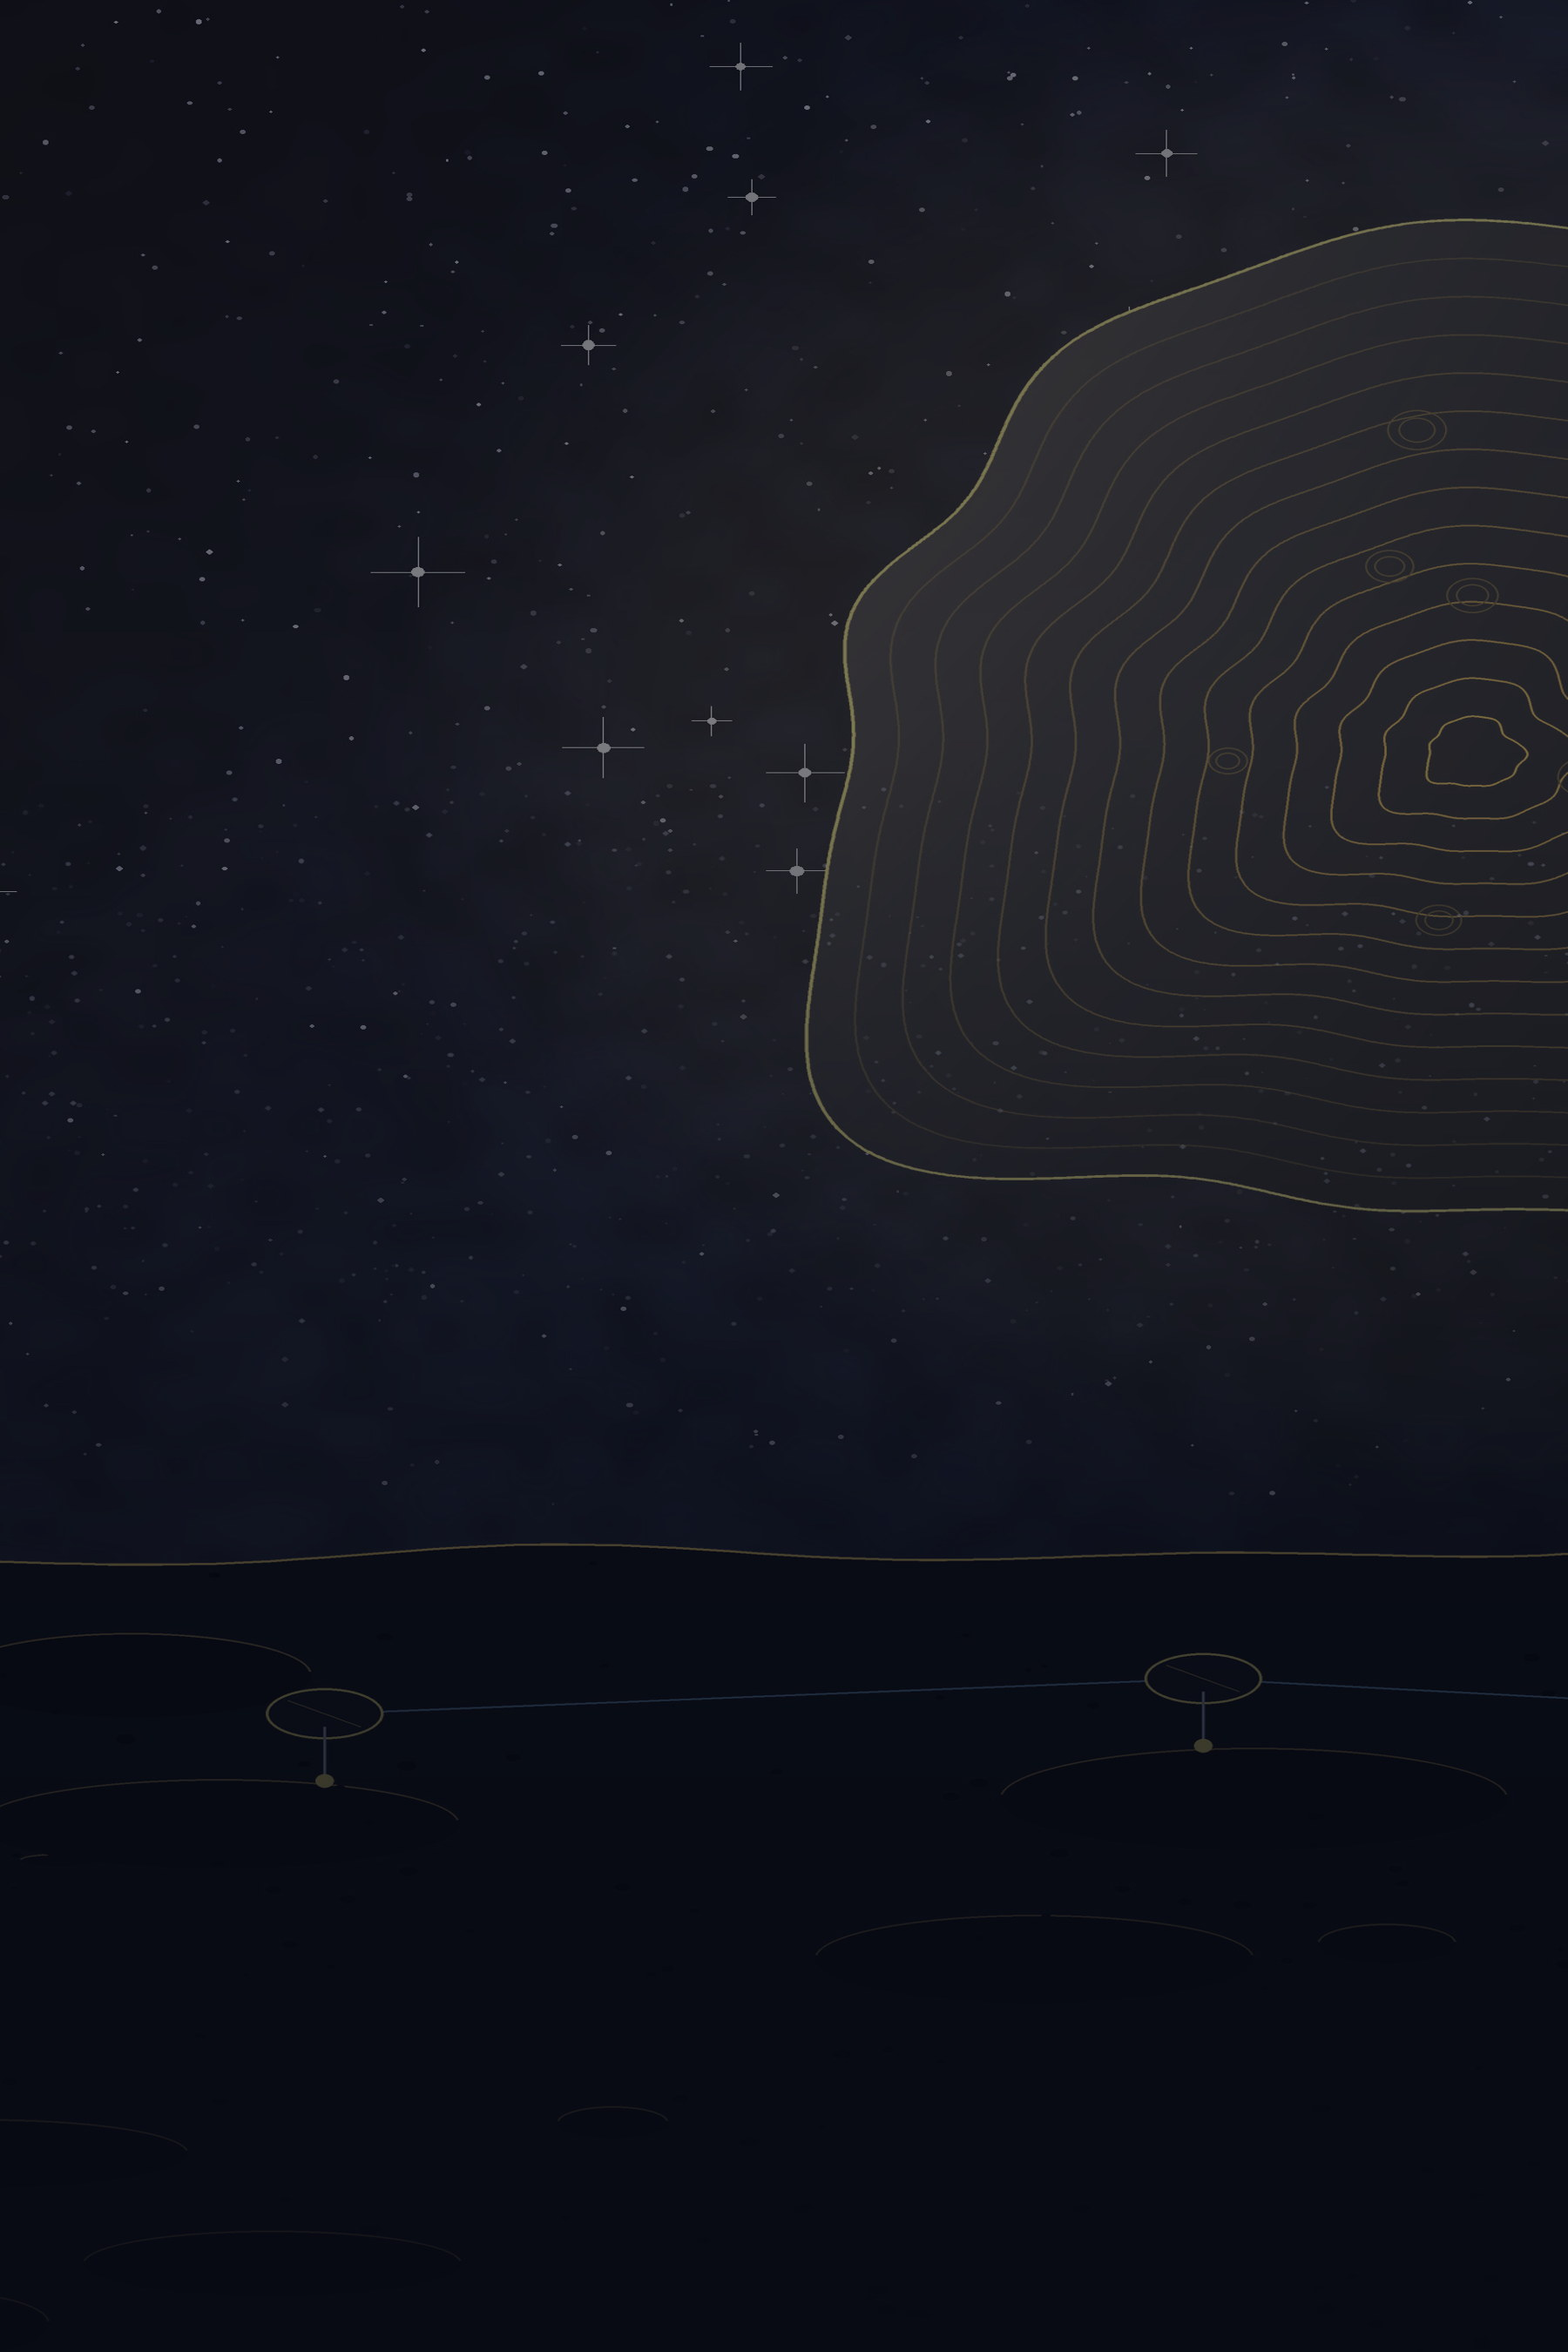
\includegraphics[width=\paperwidth,height=\paperheight]{../figures/cover_back_art.jpg}};

  % ---- title strip -------------------------------------------------------
  \node[anchor=south west,inner sep=0,text=accent] at ([xshift=0.60in,yshift=8.26in]current page.south west)
    {\fontsize{9.2}{11}\selectfont\sffamily\bfseries
     {\addfontfeatures{LetterSpace=15}THE SHAPE OF THE THREAT}};

  \fill[accent] ([xshift=0.60in,yshift=8.00in]current page.south west)
         rectangle ([xshift=5.40in,yshift=8.02in]current page.south west);

  \node[anchor=south west,inner sep=0,text=dim] at ([xshift=0.60in,yshift=7.66in]current page.south west)
    {\fontsize{9.8}{12}\selectfont\sffamily Gerald Enrique Nelson Mc Kenzie};

  % ---- blurb -------------------------------------------------------------
  \node[anchor=north west,inner sep=0,text=txt,align=left] at ([xshift=0.60in,yshift=7.24in]current page.south west)
    {\fontsize{8.1}{11.0}\selectfont\sffamily
     The catalogue knows what is out there and almost nothing about what it\\
     is. An entry carries an absolute magnitude and an orbit. It carries no\\
     size, no mass, no shape and therefore no energy and no hazard class,\\
     and the energy a defender must quote is uncertain by a factor of\\
     three for that reason alone.\\[7pt]
     This book works the chain that closes that gap --- shape to size to\\
     mass to energy to hazard class --- from first principles, and then asks\\
     where, if anywhere, a platform on the Moon earns its place in it. The\\
     answer is narrower than the question deserves and is given with its\\
     arithmetic: a fixed lunar surface array cannot find what the ground\\
     networks have not found, and cannot survey what they can find. What it\\
     can do is convert a detection into an account.\\[7pt]
     The argument is measured against the historical record rather than\\
     against a model of it: the discovery dates and the close approaches\\
     are taken from the NASA/JPL record, and the cases that were found late\\
     are worked one by one. The book also records where the proposal\\
     loses --- the thermal channel, the survey race and the census are\\
     three arguments against it, and they are stated at full strength.};

  % ---- parts -------------------------------------------------------------
  \node[anchor=south west,inner sep=0,text=accent] at ([xshift=0.60in,yshift=2.72in]current page.south west)
    {\fontsize{6.8}{8}\selectfont\sffamily\bfseries {\addfontfeatures{LetterSpace=18}INSIDE}};

  \node[anchor=north west,inner sep=0,text=txt,align=left] at ([xshift=0.60in,yshift=2.58in]current page.south west)
    {\fontsize{8.4}{11.4}\selectfont\sffamily
     I \quad The Catalogue and the Gap\\
     II \quad The Physics of Accountability\\
     III \quad The Probability Chain\\
     IV \quad Measuring Shape\\
     V \quad The Moon\\
     VI \quad The Alternatives and the Rule\\
     VII \quad Close};

  % ---- footer ------------------------------------------------------------
  \fill[dim,opacity=0.45] ([xshift=0.60in,yshift=0.92in]current page.south west)
         rectangle ([xshift=5.40in,yshift=0.93in]current page.south west);

  \node[anchor=south west,inner sep=0,text=dim] at ([xshift=0.60in,yshift=0.66in]current page.south west)
    {\fontsize{7.6}{9.6}\selectfont\sffamily
     Tico Internet LLC \quad\textperiodcentered\quad 2026 First Edition
     \quad\textperiodcentered\quad Apache License 2.0};

  \node[anchor=south west,inner sep=0,text=dim] at ([xshift=0.60in,yshift=0.46in]current page.south west)
    {\fontsize{7.6}{9.6}\selectfont\sffamily DOI 10.5281/zenodo.24517244};
\end{tikzpicture}
\null
\end{document}
